\documentclass[11pt]{book}
\usepackage[colorlinks = true,linkcolor = blue]{hyperref}
\usepackage[letterpaper]{geometry} % Custom margins
\usepackage{graphicx}
\usepackage{tabularx}
\usepackage{float}
\usepackage[spanish]{babel}
\usepackage[T1]{fontenc}
\usepackage[utf8]{inputenc}
\usepackage{remreset}
\usepackage{enumitem}
\usepackage{xparse}
\usepackage{wrapfig}
\usepackage{amssymb,amsmath}
\usepackage{tikz}
\usetikzlibrary{
  arrows,
  positioning,
  matrix,
  calc,
  decorations.pathreplacing,
  decorations.pathmorphing,
  decorations.markings,
  decorations.text,
  shapes,
  backgrounds,
  shadows,
  trees,
  fit,
  snakes,
  patterns,
  mindmap,
  intersections,
  calendar,
  plotmarks,
  spy,
  tikzmark}
  
  \decimalpoint

%%%% APRENDISAJES TEXTBOX
\tikzset{
  abstractbox/.style={
    draw=black, fill=white, rectangle, 
    inner sep=12pt, style=rounded corners,
    drop shadow={fill=black, opacity=1}
  },
  abstracttitle/.style={fill=white}
}
\newcommand{\boxabstract}[2][fill=white]{
  \begin{tikzpicture}
    \node [abstractbox, #1] (box)
    {\begin{minipage}{0.9\linewidth}
        \setlength{\parindent}{2mm} % Indentar.
        \normalfont #2
      \end{minipage}};
    \node[abstracttitle, right=10pt] at (box.north west) {Aprendizajes esperados:};
    \node[draw=none, fit=(box)] {};
  \end{tikzpicture}
}
%%%%%%%%%%%%%%%%%%%%%%%%

\makeatletter
  \@removefromreset{section}{chapter}
\makeatother
\addto\captionsspanish{\renewcommand{\chaptername}{}}
\renewcommand{\thechapter}{Unidad \arabic{chapter}}
\renewcommand{\thesection}{S\arabic{section}}
\renewcommand{\thesubsection}{L\arabic{subsection}}
\setlength{\parindent}{0pt}

%%%%%%%%%%%%% START questions env
%Idea from https://tex.stackexchange.com/a/236668/1952
\DeclareDocumentCommand\question{o}{%
    \item\IfNoValueTF{#1}{}{(#1 puntos)}}
\newenvironment{questions}[1][]{\enumerate[,#1]}{\endenumerate}
\newlist{oneparchoices}{enumerate*}{1}
\setlist[oneparchoices,1]{label=\quad\alph*), itemjoin={{\quad}}}
\newlist{choices}{enumerate*}{1}
\setlist[choices,1]{label=\quad$\square$, itemjoin={{\\}},leftmargin = 1cm}
\newcommand{\choice}{\item}
%%%%%%%%%%%%% END questions env
\makeatletter
  \@removefromreset{section}{chapter}
\makeatother

\begin{document}
\pagestyle{empty}
\newgeometry{letterpaper,left=15mm,top=50mm,bottom=0mm} % Custom margins
\begin{center}
  {\Huge Qu\'imica}\\
  \vspace{2cm}
  \normalsize
  \textbf{\large Cuaderno de trabajo}\\
  para los alumnos de 3$^\circ$ de  Secundaria\\
  en el curso durante el ciclo escolar\\
  \textbf{2022-2023}\\
  \vspace{2cm}
  \small POR\\
  \Large J. C. Melchor Pinto\\[0.5em]
  \normalsize Profesor de asignatura en\\
  \vspace{1cm}
  
\includegraphics[width=4cm]{./Unidad 2/Images/LOGO_RDS_nobg}
\end{center}
\vspace{1cm}
%\include*{Functional/TitlePage}
\hspace{-16mm}
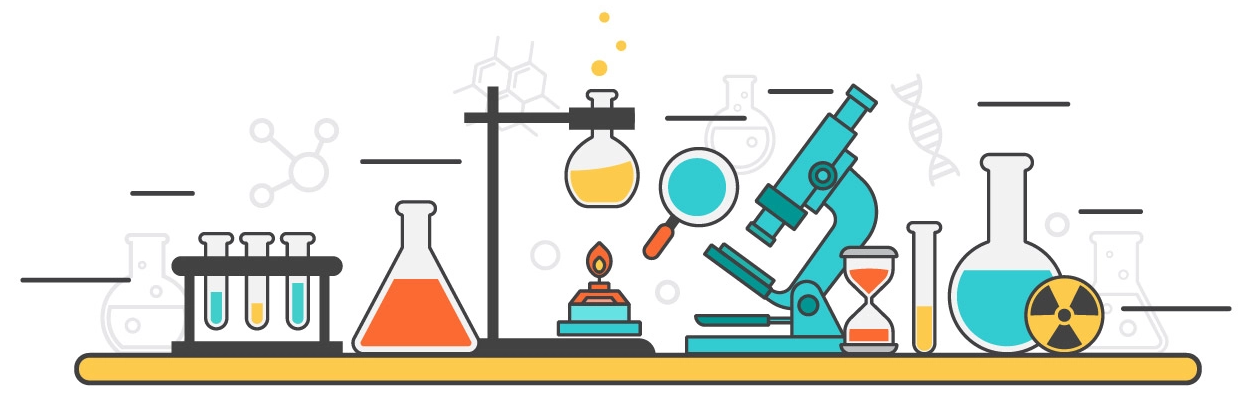
\includegraphics[width=\paperwidth]{./Unidad 2/Images/cover_bg}
\restoregeometry
\tableofcontents
\chapter{}
\section{Nuestro mundo químico}
\subsection{La química en tu vida y el medio ambiente }

\section{Los materiales, las sustancias y sus propiedades}
\subsection{¿Cómo sabemos que un material es distinto de otro?}
\subsection{¿Cómo podemos medir las propiedades de los materiales?}
\section{Relación entre propiedades de las sustancias e intercambios de energía}
\subsection{¿Cómo utilizamos energía para analizar sustancias?}

\section{Mezclas: propiedades y métodos de separación}

\subsection{Propiedades y clasificación de las mezclas}

\section{Mezclas y sustancias contaminantes}
\subsection{¿Cómo detectamos y prevenimos la presencia de sustancias nocivas en el medio ambiente?}

\subsection{Métodos de separación de mezclas}

\section{Sustancias elementales y sus propiedades}
\subsection{¿Hay sustancias más simples que otras?}
\subsection{Regularidades en las propiedades de las sustancias elementales}

\chapter{}

\section{La estructura de la materia y sus modelos}
\subsection{¿Cómo los átomos y las moléculas hacen distintas a las sustancias?}
\subsection{¿Qué hace a un átomo diferente de otro?}
\subsection{¿Cómo estudiamos a los átomos de manera experimental?}

\section{Composición y estructura de distintos tipos de sustancias}
\subsection{¿Qué tipos de partículas se forman al combinar los átomos?}

\section{Moléculas de importancia para la vida}
\subsection{¿Qué moléculas nos constituyen?}

\section{Relaciones entre la estructura y las propiedades de las sustancias}
\subsection{¿Cómo interaccionan las moléculas?}
\subsection{¿Cómo se explican y predicen las propiedades de las sustancias?}

\section{Reacciones químicas en nuestro mundo}
\subsection{¿Cuál es la evidencia de que las sustancias reaccionan unas con otras?}

\section{Recombinaciones atómicas}
\subsection{¿Cómo representamos las reacciones químicas?}
\subsection{¿Qué cambia y qué se conserva durante las reacciones químicas?}

\section{Cantidad de las sustancias}
\subsection{¿Cómo determinamos la cantidad de las sustancias?}
\subsection{Cantidad de las sustancias en reacciones químicas}


\chapter{}

\section{Un mundo de reacciones químicas}
\subsection{¿Cómo nos afectan las reacciones químicas?}
\subsection{¿Cómo aprovechamos las reacciones químicas?}

\section{Energía y reacción química}
\subsection{¿Cómo se transfiere energía durante las reacciones químicas?}
\subsection{¿Por qué se transfiere energía durante las reacciones químicas?}

\section{La energía química en nuestras vidas}
\subsection{¿Cuáles son los beneficios, costos y riesgos de usar energía química?}

\section{Aporte calórico de los alimentos}
\subsection{¿De dónde proviene la energía que necesitamos para vivir?}

\section{Rapidez de reacción}
\subsection{¿Qué factores afectan la rapidez de las reacciones químicas?}

\section{La rapidez de reacción y el modelo cinético de partículas}
\subsection{¿Cómo explicamos diferencias en la velocidad de reacción?}

\section{Utilidad de controlar la rapidez de las reacciones}
\subsection{¿Cómo controlamos y aprovechamos la velocidad de reacción?}

\end{document}






